\chapter{Prestudy}
Given the problem Vitensenteret presented to the group, it was necessary for the group to look at solutions to similar problems and conduct a brainstorming session to come up with ideas. It was also important to gather knowledge about different technologies and frameworks as well as different development methods. This chapter will elaborate on the different ideas, technologies and development methods that were considered for this project.

\section{Ideas for the application}
The first impression of the problem was that Vitensenteret already had a clear vision for the application, but the first meeting between the group and the staff at Vitensenteret proved otherwise. Vitensenteret told the group that they wanted a mobile application, but they did not specify how they wanted it to be. Although they did not specify how they wanted the application to be, they did come with a few ideas to the group. These ideas were considered and some of them were even used in the final version of the application. The next sections explain sources of inspiration and the ideas that were considered for the application.\\

\subsection{Similar applications}
To find inspiration for the application that was to be made, the group searched for similar applications. This subsection will go through the different applications that were found and how they inspired the group.

\subsubsection{Science Museum in London}
The Science Museum in London \cite{smlondon} had quite many applications for the group to look at. One of the applications involved using beacons to interact with the exhibition in London\cite{smlondon1}. The group was intrigued by this idea and started to look more into the beacon technology. Read more about beacons in section 2.1.4.\\
\\
Another application let the user design their own space rover\cite{smlondon2}. This gave the group an idea to use the same concept, but in a different manner. The group saw the opportunity to use this concept as a rewarding concept in the application. Read more about rewards in the application in section 2.1.7.

\subsubsection{American Museum of Natural History}
The American Museum of Natural History\cite{amnh} did also have several applications, one of which the group found interesting. It was meant to be a guide throughout the exhibition, and to give the user a new experience in the museum\cite{amnh1}. This gave the group a similar idea. Read more about this concept in section 2.1.6.

\subsection{Virtual reality}
Virtual reality is a technology the team thought would bring more customers to Vitensenteret, in that the group considered the technology itself  appealing by the masses. The idea was to make an application which takes the user on a trip through the universe, describing and visually displaying objects like the earth, stars, galaxies and more, and comparing the properties of these objects like for instance the size and weight. This could give the user, especially the younger ones, a sensational experience and a new perspective of how big the universe is. Using virtual reality for this could be a good idea because it further immerses the user into the environment of the application. To execute the idea the group had, knowledge about 3D-modeling was required\cite{virtualreality}. 

\subsection{Augmented reality}
Vitenseteret suggested that the group could use augmented reality in our project. Their reasoning was that it was a relatively new technology and that it could be innovative to use at a museum. The concept of augmented reality is capturing the real-world environment with a camera, and augmenting it with software. For instance, through the application the user could view objects through the camera that one otherwise would not see in the real world. This kind of augmented reality application would require knowledge about 3D-modeling.

\subsection{Beacons}
The customer wanted the group to make a cool application, and preferably with new technology. This made the group think of beacons. Beacons are small Bluetooth-devices that constantly sends out data to tablets and smartphones. The data sent by the beacons varies and can trigger actions on the device that receives the data. This action can be anything from opening a web page to have an app that does a specific thing when it receives the data\cite{whatisbeacon1}\cite{whatisbeacon2}.\\
\\
The use of beacons could connect the application to the exhibition in the sense that the users have to look for the different beacons in the exhibition to trigger actions in the application.

\subsection{Minigames}
The idea to structure the application as a series of minigames came to the group while brainstorming in the exhibition. Because the different sections in the exhibition have different themes, the group thought of making different minigames that fit the different themes of the exhibition. 

\subsection{Exhibition guide}
The idea to make a guide through the exhibition is quite similar to the minigames-idea. The group got this idea from the staff at Vitensenteret, as well as from the application from the American Museum of Natural History. The application will take you through the museum, visiting all parts of the exhibition. One idea was to make the application a story that guided the user through the museum. The group though this could make the application more interesting and hopefully trigger the curiosity of the user, which in turn would make the user want to go through the whole museum.

\subsection{Rewards}
In order to make the application more appealing towards the targeted audience, the group considered adding or implementing different kinds of rewards.\\
\\
The group discussed the possibilities for physical rewards or discounts in Vitensenterets gift shop with Vitensenteret. The main idea here was that the children who finished the application could show their smartphone to the staff managing the gift shop and get either a small box of candy or discount on a small item in the gift shop.\\
\\
Having rewards in the application itself was also considered. The idea was that whenever progress was made in the application, the user would get something in the application, e.g. parts for a robot or parts for a map. When all parts have been completed, the user has enough parts to either make a robot or to complete a treasure map.

\section{Frameworks and Technologies}
All the ideas that were considered for the application required different technology. This made the group explore different technologies which made the different ideas possible. This subsection introduces the different technologies and explains which problem they could solve.

\subsection{Native platform}
The first technology considered was based on development for the native platforms. The native platforms are Apple's iOS for iPhones, Google's Android and Microsoft's Windows Phone.

\subsubsection{iOS}
Native development for iOS can be done with multiple programming languages, but is mainly done in Objective-C and Swift\cite{ios2} \cite{ios3}. To develop native iOS applications, it is necessary to have a device running OS X, Apple's computer operating system, with Xcode installed. It is not possible to develop Native iOS application without this\cite{ios1}.\\
\\
Seeing that Apple's iPhone held a big share of the Norwegian smartphone market, it would make sense to develop an application for this operating system. Another good thing about iOS development was that it supported development with beacons, virtual reality, and augmented reality.\\
\\
One problem with this solution was the fact that it excluded the other platforms unless applications were developed for the other platforms as well. Another problem was, as mentioned above, that you needed special tools to be able to develop native applications for iOS.


\subsubsection{Android}
Another possibility was to develop a native application for the Android platform. This could be done using Java, C, and C++, although Java was the promoted programming language by Google\cite{android1}. Native application development for Android could be done using any operating system, this included Windows, Linux, and OS X.\\
\\
Android, like iOS, held a big share of the Norwegian smartphone market. It would therefore also make sense to develop for the Android operating system. Unlike iOS application development, Android application development did not require any special tools. All that was needed were a JDK, an SDK, and an IDE. Native development for Android supports beacons, virtual reality, and augmented reality. \\
\\
The problem with developing a native Android application was the same as with iOS; the other platforms would get excluded.

\subsubsection{Windows Phone}
Native application development for Windows Phone could be done using C\# or Visual Basic for the code part and XAML for the visuals. The tools for making Windows Phone applications were most functional when using the Windows desktop operating system, but Microsoft has made it possible to make applications on UNIX based operating systems as Linux and OS X.\\
\\
Unlike Android and iPhone, there were not many Windows Phones on the market, and it was therefore not very attractive to develop for Windows Phone. Development of native Windows Phone applications on other desktop operating systems could be complicated. It could therefore be hard to develop native Windows Phone applications.

\subsection{Google VR}
The Google VR SDK was a software development kit provided by Google for the development of Virtual reality applications for both iOS and Android. The SDK allowed for development of virtual reality applications for two of Google's own virtual reality devices; Google Cardboard and Google Daydream\cite{daydream}\ cite{googlevr}.\\
\\
Google Cardboard was Google's cheap virtual reality device, which allowed anyone with a smartphone to develop and experience virtual reality applications. It was cheap and far from the best quality on the market.\\
\\
Google Daydream was Google's high-end virtual reality device. It was more expensive than Google Cardboard, but the quality was better. Google Daydream, like Google Cardboard, used a smartphone to portray the virtual reality. Google Daydream also came with some extra features compared to the Google Cardboard. It came with a controller that made it easier to navigate and control in the virtual environment. 

\subsection{Cross platform}
An option to developing native applications was developing cross platform applications. There were many frameworks and libraries that enabled cross platform development, some of which were considered for this project.

\subsubsection{Xamarin}
Xamarin was an application development platform which enabled making cross-platform applications. It was based on the programming language C\# and it could be used to make applications for Android, iOS, and Windows Phone\cite{xamarin}.\\
\\
Xamarin was compiled for native performance, which cannot be achieved with other cross-platform development tools. It also utilizes native libraries and API's. So every library or API that is made for either Android, iOS or Windows Phone can also be used by Xamarin apps. Xamarin is a tool that costs money unless the project it is being used to develop for is open-source.

\subsubsection{Cordova}
Cordova was a free and open-source framework for cross-platform application development.\cite{cordova} It was issued under The Apache Software Foundation, which supports open-source development. Cordova was based on wrapping web technologies in a native wrapper. This enabled an application developer to use HTML, CSS, and JavaScript to develop an application, and then Cordova wrapped it in the code for the platforms wanted.\cite{cordova2} It was possible to make applications for several different platforms, including Android, iOS, Windows Phone, and others. Cordova had support for plugins which enabled native functionality. Developing with Cordova gave the applications some restrictions. The main restriction was performance.\cite{cordova3} Cordova did also have plugins with support for iBeacons\cite{ibeacon_plugin}, and Eddystone\cite{eddystone_plugin} beacons.

\subsubsection{Ionic}
Ionic is an open source HTML5 mobile application development framework. It builds on top of Cordova and uses AngularJS. Ionic can be thought of as a front-end user interface framework that handles the look and feel of the user interface interactions. The functional part of Ionic comes from AngularJS, but AngularJS is not required for Ionic to function. Without AngularJS, Ionic consists of CSS and Sass modules which can be used for designing elements of the application.\cite{ionic}\\
\\
Ionic is a framework that supports developing applications with MVC architecture. This is because of AngularJS support, which is a Model View Whatever (MVW) architecture, that supports all Model View architectures. One of the key features of Ionic was that is makes standardized design easier. Applications developed with Ionic will not preform as good as native application, but for the sake of this application it preforms very good. 
\cite{ionic2}\cite{ionic3}

\subsection{Beacons}
Amongst multiple choices of beacon technology standards in the industry, the group found two standards more attractive.
\\
\\
\textbf(iBeacon) was a beacon standard developed by Apple. This technology standard allowed mobile applications for both Android and iOS to listen for Bluetooth-signals broadcasted with it.
\\
\\
\textbf{Eddystone} was Google's new open source beacon standard, which deviated from Apple's iBeacon standard. It could transmit larger data packages, which meant the beacon could send an external URL, from which the user could download content instead of installing a specific app. This opened for a variety of possibilities, where the iBeacon standard came short in comparison, since it only can broadcast an identifier, which an application would need to read in order to do an operation. With Eddystone you can download content(e.g. a website) from the url provided in the package.



\section{Development methods}
To find a development method that fit the project, the team made an effort in considering several development methods.

\subsection{Scrum}
Scrum is an agile and iterative  development method. The method is designed to help small teams develop complex products. Scrum is mostly used in the technology sector, but it is also found elsewhere. A scrum team usually consists of around seven people who work together.  One of the mantras of scrum is “inspect and adapt,” scrum teams are known for being determined about constantly improving their work process and the product they are developing.\cite{agilelearning}

\subsubsection{Sprints}
In scrum the team works together in what is called sprints. A sprint is a set period of time, where specific work has to be completed and ready for review. The duration of the sprint, as well as the planned work is determined together by the team. Once the team reaches a consensus for the duration of the spring, each sprint should be of the same length. A sprint can typically last from one day to 30 days. A project maneged by scrum consists of many sprints, where one sprint builds upon the previous sprint.\cite{agile}

\subsubsection{Roles}
Scrum requires the team to be divided into three different roles: product owner, scrum master and development team. \\
\\
\textbf{Product owner:} The product Owner holds the vision of the product, and is the voice of the customer. The product owner is responsible for the scrum team and that they do what they are supposed to. In addition to being resource to the development team by answering different kinds of questions.\cite{agilelearning}\\
\\
\textbf{Scrum master:} The scrum master is the expert on scrum and adviser. The scrum master helps the team apply scrum and helps the team overcome any kinds of obstacles or interferences that might occur on the road. It is important to note that the scrum master is the team's boss, the scrum master is only there to help the team organize the project and preform better.\cite{agilelearning}\\
\\
\textbf{Development team:} The development team consists of all the developers. They are the ones who have full control and authority over what is done and what is going to be done. The developer team is responsible for all the actual work, including prototyping, deigning, developing, testing and so on.\cite{agilelearning}

\subsubsection{Scrum cycle}
The standard Scrum cycle is to have daily meetings, with each team member presenting their work, potential problems, and so forth. The meetings also have a very specific procedure, to assure the maximum efficiency. In the end of each sprint, there is also a sprint reflection meeting where the team discusses what could have been done better and the current situation of the development process. Then the outcome of each sprint is presented for the customer, and the team is open for feedback.\cite{agilelearning}\\
\\
Figure \ref{fig:Scrum} illustrates the cycle of a sprint. Where the product backlog is an overview containing all the different tasks that has to be done on order for the project to be complete. The sprint backlog are the task taken from the product backlog, and are the task that are supposed to be completed within a given sprint.

\begin{figure}[H]
\centering
    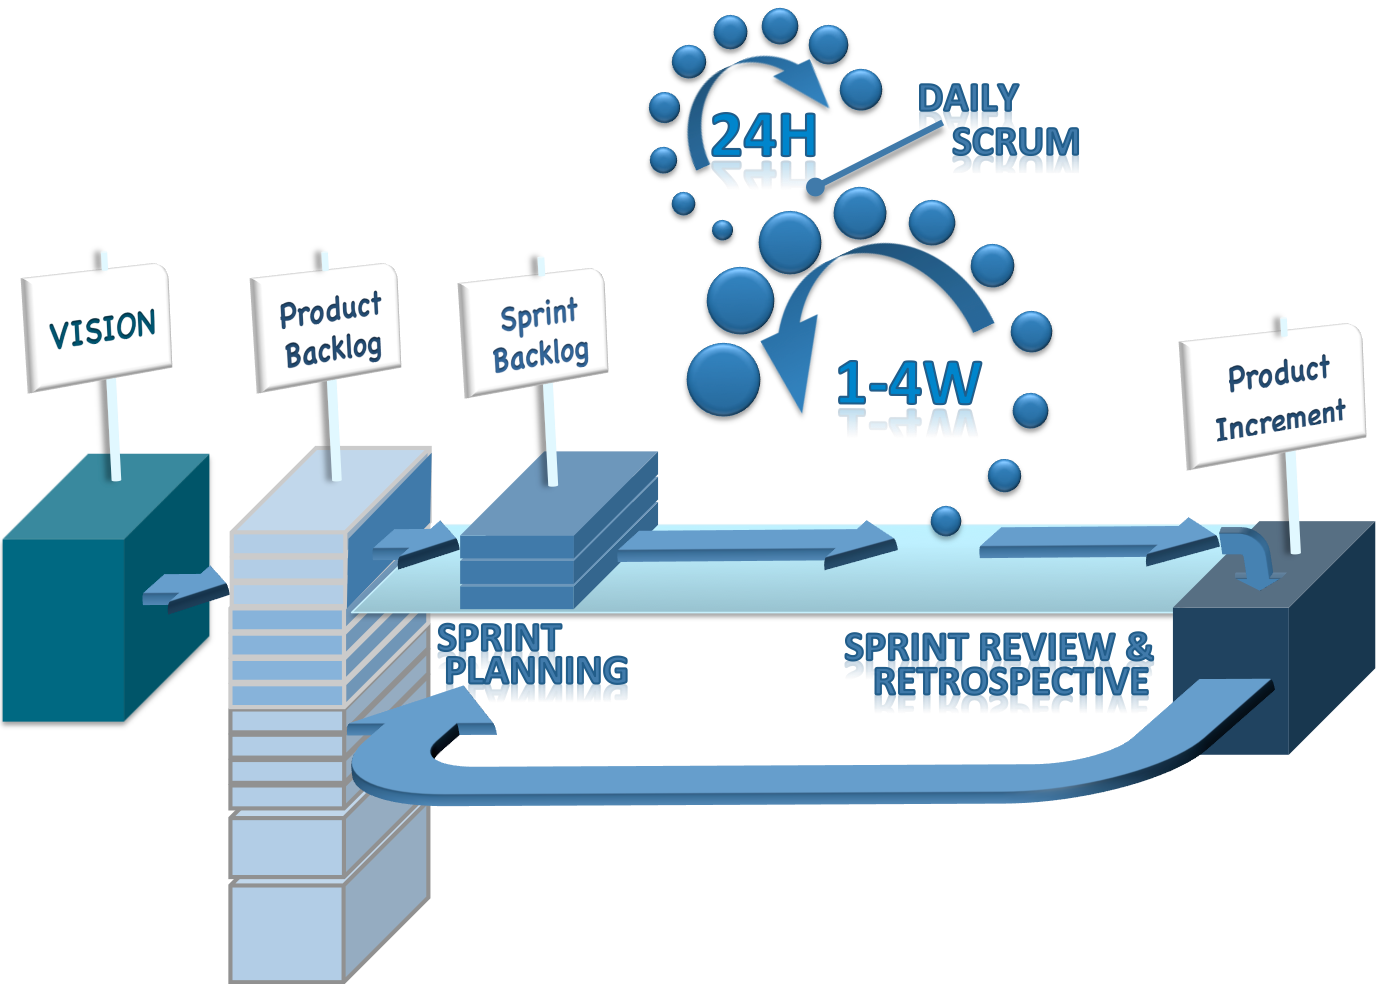
\includegraphics[width=\textwidth]{images/scrum.png}
    \caption{The Scrum cycle}
    \label{fig:Scrum}
\end{figure}

\subsubsection{Reflection}
The goal with Scrum is the fact that the team can present new functionality for the customer, and get feedback throughout the development process by including the customer in the life-cycle of an iteration. This would reduce the possibility of disagreements and unsatisfied customers when the product is to be released. Another advantage about Scrum is the flexibility and freedom that comes with having a board of tasks to choose from. In some cases, a development decision makes choices for the team, for example if there is a conflict of interest in regards to dividing the workload. Scrum is often criticized for the amount of effort and knowledge required by all the members for it to be efficient. A common workaround to this is to define the contents and procedure of the meetings as it fits the team.  

\subsection{Waterfall}
The waterfall method is a development method that was very popular for a long time. It was one of the first process models to be introduced and is also known as linear-sequential life cycle model. The model is very simple to follow and use. Usually, the method consists of five stages in the following order; requirements, design, implementation, verification, and maintenance. Each phase must be fully completed in order for the next one to begin. This method is common in smaller projects where the requirements are simple and there are no uncertainties.\cite{wf}

\subsubsection{Sequential progress}
The waterfall model provides a framework that aims to complete the development cycle sequentially. It is described as sequential, in that it divides the work into phases. The standard waterfall model defines five phases: requirements, design, implementation, verification and maintenance, and is to be completed in that order. As can be seen in figure \ref{fig:Waterfall}, when all the phases are complete, then the product is finished. In contrast to the Scrum model described in the previous subsection, the waterfall model is characterized with strict planning procedures and documentation. This is because any change in the requirements or any change major correction could force the developers to redo a phase that is marked as completed, which could be expensive.\cite{wf}
\\
\begin{figure}[h]
    \centering
    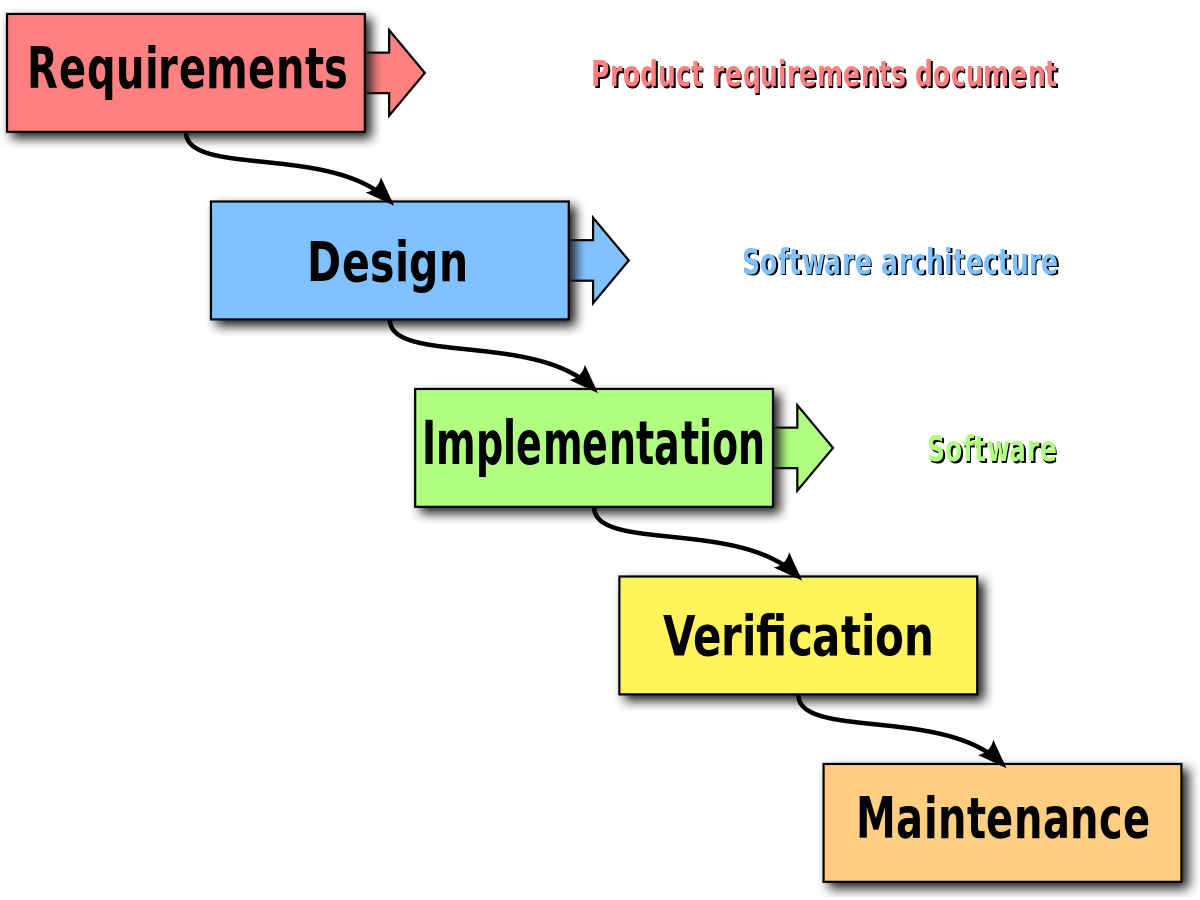
\includegraphics[scale=0.2]{images/Waterfall_model.png}
    \caption{The Waterfall method.}
    \label{fig:Waterfall}
    \cite{wf}
\end{figure}
\\
\subsubsection{Reflection}
Whilst agile development methods require good communication to be effective, the sequential waterfall model relies more on good documentation analysis than on communication. Generally, the bigger the team - the worse the communication in the team would be. By this logic, the waterfall model might be suitable for some of the big development teams. If the task is to develop a system that in any case would require a lot of analysis and documentation, the disadvantage of adding additional work in the documentation would cancel out. In the requirements phase, the development team analyzes the requirements provided by the customer. Since the customer relies on the team to accurately analyze the requirements, and since the customer is not included in the development process, the risk of surprises and unhappy customers increases with the complexity of the requirements. It could, however, work well if the requirements are static and easy to analyze. 

\subsection{Lean software development}
Lean software development was an agile software development method created by Mary and Tom Poppendieck. It was based on seven principles:\\
\\
\textbf{Eliminate waste:} Get rid of everything that did not have any value to the customer, e.g. partially done work.\\
\\
\textbf{Amplify learning:} The development process should be customized to amplify learning for the developers. This was done by using short iteration cycles and focus on testing code as soon as it was written.\\
\\
\textbf{Decide as late as possible:} Delaying decisions as much as possible to be able to make decisions based on facts and not uncertain assumptions and predictions. This would result in better decisions being made.\\
\\
\textbf{Deliver as fast as possible:} If the project is delivered sooner, it will result in getting feedback earlier than a late delivery.\\
\\
\textbf{Empower the team:} Instead of managers telling the workers how to do their work, the roles were turned. The managers were taught to listen to developers, so that they better can explain what actions should be made.\\
\\
\textbf{Build integrity in:} The customer needs to have insight and influence in how the system is advertised, delivered, deployed, accessed, how intuitive it was to use, price and how well it solved the problem. This would give the customer a comprehensive experience of the system.\\
\\
\textbf{See the whole:} Decompose big tasks in the project into smaller tasks. This made it easier to find and eliminate defects.

\subsection{Pair programming}
Pair programming is an agile development technique in which two developers work together on a single workstation. The two developers take turns writing code while the other developer reviews each line of code that is being written. The programmer is often called ``the driver" and the reviewer is often called ``the observer". The driver's main role is simply just to write the code and completing the current task. While the observer is responsible for verifying the code. In addition to taking likely future problems into account, by suggesting improvements to the code.\cite{pp}\\
\\
With this programming method comes many advantages. Research shows that pairs tend to spend 15\% more time on programming than individuals. However, the result is usually a program with 15\% less unwanted features.\cite{pp2} Today, one of the biggest expenses in the digital world in is solving and repairing software problems. Pair programming results in code with higher quality which again results in a reduction of resources spent on repairing software.\\
\\
Research has also shown that other advantages of pair programming are increased design quality. Two programmers working together are more likely to come up with a more future-oriented solution. It is also shown that programmers enjoyed their work more while working in pairs. Since knowledge is constantly shared between the developers it is also more likely that the learning outcome is much bigger than working alone. 

\subsection{D3: Design Driven Development}
D3 is an agile approach to development. It adds another dimension to the software development by making innovation, design and usability central in the development process. D3 turns design practices into games to bring different people with different sets of skills together to make design decisions together\cite{designdriven3}. The games are put into five different categories\cite{designdriven2}:\\
\\
\textbf{Startup:} These were games designed to help the team find the motivation for the project.\\
\\
\textbf{Understand:} These were games developed to make the team understand the existing system and problems by exploring the domain, business, customer, users and context.\\
\\
\textbf{Question:} It is important to ask questions to be innovative. The games in this category were designed to make the team question the existing business models, systems and processes.\\
\\
\textbf{Design:} Explore some of the elements of design, e.g. interaction and information.\\
\\
\textbf{Experience:} Design was not an one time project, but a process of improvement and refinement.\\
\\
This is an agile development method that resembles Scrum and Extreme programming in its iterative ways, but instead of bringing agility to overall management, estimation, and planning, or to engineering activities, D3 brings agility to solution design and innovation\cite{designdriven1}. See Figure \ref{fig:d3} for a visual picture of how D3 functions as an agile development method.\\
\\
\begin{figure}[h]
    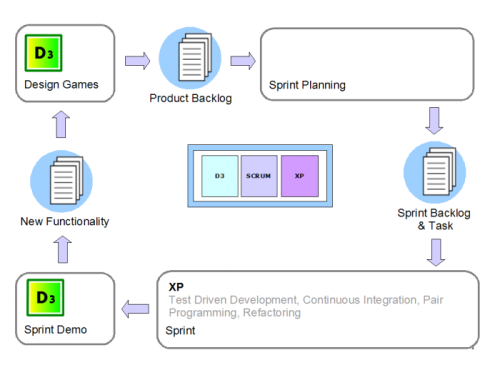
\includegraphics[width=\textwidth]{images/Agile_D3_small.png}
    \caption{The D3 method}
    \label{fig:d3}
\end{figure}



\subsection{Extreme programming}
Extreme programming (XP) is an agile development that defines as the set of rules that certain values, namely simplicity, communication, feedback, respect, and courage. XP is also characterized by it's incremental and iterative development in which there is a new version/release on every iteration.  \cite{XP_desc}.

\subsubsection{User Stories}
In the planning phase, the customer provides User stories to the developers. User stories consist of 3 sentences of text and briefly describes a feature. The description should avoid technical details such as technology and algorithms, but should contain enough information such that the developers can roughly estimate the implementation time in terms of weeks. The user stories are also used to create test scenarios for acceptance tests. When it is time to implement a user story, the development team would contact the customers and get a full description of the requirements. \cite{XP_UserStories}

\subsubsection{Iterative development}
The work is divided into about a dozen iterations of 1 to 3 weeks in length. The iteration length is to be kept constant throughout the project because it makes measuring progress and planning more simple and reliable. All the code needs unit tests, and all the unit tests must be passed before it can be released for customer approval. There is also rules for iteration planning, acceptance testing, changes in terms of architecture and time estimates (spikes). 

\subsubsection{Customer involvement}
One of the biggest requirements for XP to work is customer presence in the project. Unlike Scrum, where the developers and customers meet in between each iteration, in XP, the customer is required to be present every day as every phase in the standard XP requires customer involvement. For this reason, XP might be more suitable when the customer is located close by and has the time and will to be involved in such a process, than if the customer is busy, and is located far away. 

\subsubsection{Considerations}
To have the customer present each day of the development process would require the team to go to Vitensenteret every work-day, and work from there. For that to happen, the team would have to ask for an office there, and hope that Vitensenteret had the time to attend to the process and deliver feedback every day. It was already established that the team and Vitensenteret would meet every other week. \cite{XP_iterativedevelopment}